\hypertarget{_base___dados_8cpp}{}\section{src/\+Base\+\_\+\+Dados.cpp File Reference}
\label{_base___dados_8cpp}\index{src/\+Base\+\_\+\+Dados.\+cpp@{src/\+Base\+\_\+\+Dados.\+cpp}}


A base de dados é uma estrutura que armazena algumas impressões digitais em uma estrurura.  


{\ttfamily \#include \char`\"{}../include/\+Base\+\_\+\+Dados.\+h\char`\"{}}\newline
{\ttfamily \#include \char`\"{}opencv2/opencv.\+hpp\char`\"{}}\newline
{\ttfamily \#include $<$fstream$>$}\newline
{\ttfamily \#include $<$iostream$>$}\newline
Include dependency graph for Base\+\_\+\+Dados.\+cpp\+:\nopagebreak
\begin{figure}[H]
\begin{center}
\leavevmode
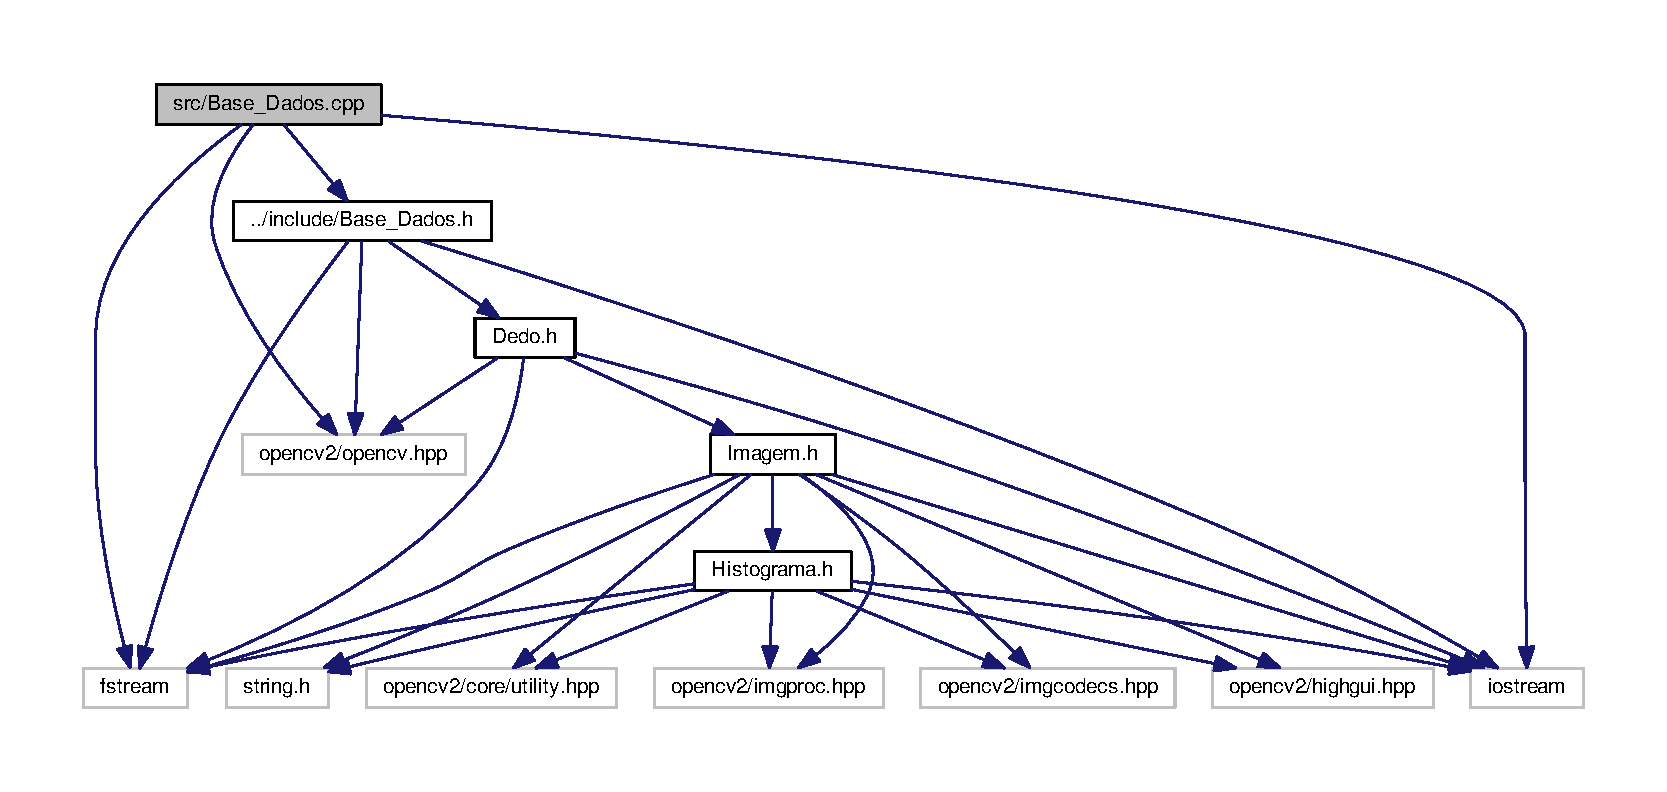
\includegraphics[width=350pt]{_base___dados_8cpp__incl}
\end{center}
\end{figure}


\subsection{Detailed Description}
A base de dados é uma estrutura que armazena algumas impressões digitais em uma estrurura. 

\begin{DoxyAuthor}{Author}
Douglas Venâncio Filipe Pena Marco Antonio 
\end{DoxyAuthor}
\begin{DoxyDate}{Date}
2018-\/07-\/01 
\end{DoxyDate}
